\documentclass[10pt, conference]{IEEEtran}

\usepackage[pdftex]{graphicx}
\usepackage[cmex10]{amsmath}
\usepackage{amsfonts}

\usepackage{color}
\usepackage{hyperref}
\hypersetup{colorlinks=true,
    linkcolor=blue,
    citecolor=blue,
    filecolor=blue,
    urlcolor=blue,
    unicode=false}
\urlstyle{same}

\usepackage{tabularx}
\usepackage{booktabs}
\usepackage{siunitx}
\usepackage{subfig}
\usepackage{paralist}
\usepackage{colortbl}
\usepackage{listings}

\usepackage{enumitem}
\usepackage{pgfplots}

\newif\ifcomments\commentstrue

\ifcomments
\newcommand{\authornotation}[3]{\textcolor{#1}{[#3 ---#2]}}
\newcommand{\todo}[1]{\textcolor{red}{[TODO: #1]}}
\else
\newcommand{\authornotation}[3]{}
\newcommand{\todo}[1]{}
\fi

\newcommand{\wss}[1]{\authornotation{blue}{SS}{#1}}
\newcommand{\ms}[1]{\authornote{cyan}{MS}{#1}}

\newcommand{\progname}{SFS}
\newcommand{\colAwidth}{0.13\textwidth}
\newcommand{\colBwidth}{0.84\textwidth}

\begin{document}

\title{A Software Engineering Capstone Infrastructure that Encourages Spreading
Work Over Time and Team}

\author{\IEEEauthorblockN{}
\IEEEauthorblockA{}

% \author{\IEEEauthorblockN{Spencer Smith, Christopher Schankula, Lucas Dutton and Christopher Anand}
% \IEEEauthorblockA{Computing and Software Department\\
% McMaster University, Canada\\
% Email: smiths@mcmaster.ca, schankuc@mcmaster.ca, duttonl@mcmaster.ca, anandc@mcmaster.ca}

% \and
% \IEEEauthorblockN{Sumanth Shankar}
% \IEEEauthorblockA{Mechanical Engineering Department\\
% McMaster University, Canada\\
% Email: shankar@mcmaster.ca }
}

\maketitle
  
\begin{abstract}

How can instructors facilitate spreading out the work in a software engineering
or computer science capstone course across time and between team members?
Currently teams often compromise the quality of their learning experience by
frantically working before each deliverable.  Some team members further
compromise their own learning, and that of their colleagues, by not contributing
their fair share to the team effort. To mitigate these problems, we propose
using a GitHub template that contains all the initial infrastructure a team
needs, including the folder structure, text-based template documents and
template issues. In addition, we propose each team begins the year by
identifying specific quantifiable individual productivity metrics for
monitoring, such as the count of meetings attended, issues closed and number of
commits.  Initial data suggests that these steps have an impact.  In 2022/23 we
observed 50\% of commits happening within 3 days of due dates.  After partially
introducing the above ideas in 2023/24, this number improved to 37\%. To measure
the fairness of how work is distributed between teammates, we consider two
fairness metrics: Jain's fairness index, and our own fairness measure based on
the disparity between number of commits between all pairs of teammates.  Going
forward we propose an experiment where commit data and interview data is
compared between teams that use the proposed interventions and those that do
not.

\end{abstract}

\begin{IEEEkeywords}
software engineering; capstone; template repository; productivity measures;
fairness metric
\end{IEEEkeywords}

\section{Introduction} \label{SecIntro}

The workload for a software engineering or computer science capstone team
project is often unevenly distributed over time and between team members.  Teams
typically work in frantic bursts of activity right before a deadline and then
cease almost all activity until their next deadline.  These work habits
compromise the learning objectives of the course because the students do not
have time to properly plan their activities or reflect on their work.  The
uneven distribution of effort between team mates is also problematic.  Some
students take on an unfair share of the work, causing them stress and possibly
hurting their experience in other courses, while those investing less effort
miss important learning opportunities.  How can instructors mitigate these
problems?

To address the uneven distribution of work, we need to first think about why the
problems exist.  A student project is not the same environment as the workplace.
Students are often learning the content just before applying their knowledge.
Since they are doing a capstone project for the first time, students might
struggle with determining the expectations; they might not know where to start.
Moreover, team members cannot be fired or moved to another project for poor
performance.  Peer pressure and the prospect of uncomfortable social
interactions can make it challenging for someone to take charge of their group,
or to criticize other group members. %any citations on these challenges?

% What can instructors do to help the students? How can they encourage the
% students to focus their efforts?  Instructors control the organization,
% structure and content of their course, and they control the rules for awarding
% grades to students. An uneven workload distribution over time and between
% team-members can potentially be improved by the instructor providing as much of
% the mundane project infrastructure as possible to save student time and to
% clearly show expectations. Furthermore, instructors can use grades to encourage
% participation by all team members.

For saving the student's time and clearly showing expectations, we suggest
requiring all capstone teams to start from the same GitHub template repository.
The template repository is populated with ....  Citations on this topic. Too much freedom in decision making can be paralyzing for a new team.  They don't know where to begin.  By making the infrastructure decisions for them, they can focus on their project.

An even workload between teammates can be improved by becoming aware of
potential problems as early as possible. Decide before things get ugly.
Citations.

In Section~\ref{SecInfrastruct} we describe the baseline structure of the
capstone course that we have modified with two interventions: 1) a template
repository; and, 2) explicit quantifiable team contribution measurement. We
follow this with some encouraging preliminary data from when we partially
introduced the two interventions into the course (Section~\ref{SecPrelimData}).
We then describe our proposed approach for collecting more detailed data to
judge the effectiveness of the proposed interventions
(Section~\ref{SecProposedExperiment}). The presentation of the proposed
experiment includes discussion of threats to validity.

\section{Baseline and Proposed Infrastructure} \label{SecInfrastruct}

The infrastructure described here matches the final year SE capstone course at
[Redacted]. %McMaster University 
This course is currently delivered to 150 students divided into 29 groups of
4--5 members. Teams are provided with a list of curated software development
projects from academia and industry. Teams can also propose their own projects.
Most projects have a supervisor/client that the team can meet with to discuss
their project.  In cases where there is no supervisor, the team still needs to
explicitly identify the stakeholders for the project.

\subsection{Structure and Timeline} \label{Sec_Structure}

Figure~\ref{Fig_VModel} show the V-model~\cite{ForsbergAndMooz1991} structure of the
capstone course. The documents created include the Software Requirements
Specification (SRS) and various Verification and Validation (VnV) plans and
reports. Due to time constraints not all artifacts of the V-model are produced.
Those that are created are circled with red ellipses, along with an annotation
showing the week number where the artifact is due for a full year (26 week)
course. The week is when the Revision 0 draft of the document is due.  Almost
all documents also have a second revision (Rev1 Doc) that is due at the end of
the course (Week 26). The iteration allows students to take the formative
assessment for Rev 0 to produce a higher quality document for their summative
review. In recognition of the value for teams of ``getting their hands dirty'',
a Proof of Concept (POC) Demo is scheduled for week 10. During this demo the
teams demonstrate the aspect of their project that is of most concern for
feasibility of the project, providing an opportunity to revise the project scope
if necessary. The Rev0 demo is expected to show off the final and complete
product. The teams rarely achieve this, but the push for Rev0, together with the
feedback they received, allows them to improve their software for the final demo
(Rev 1 demo). The structure of the course is stable, having been offered in this
form for four years. The interventions described in the next sections are in the
context of this structure. 

\begin{figure}[h!]
  \begin{center}
    {
      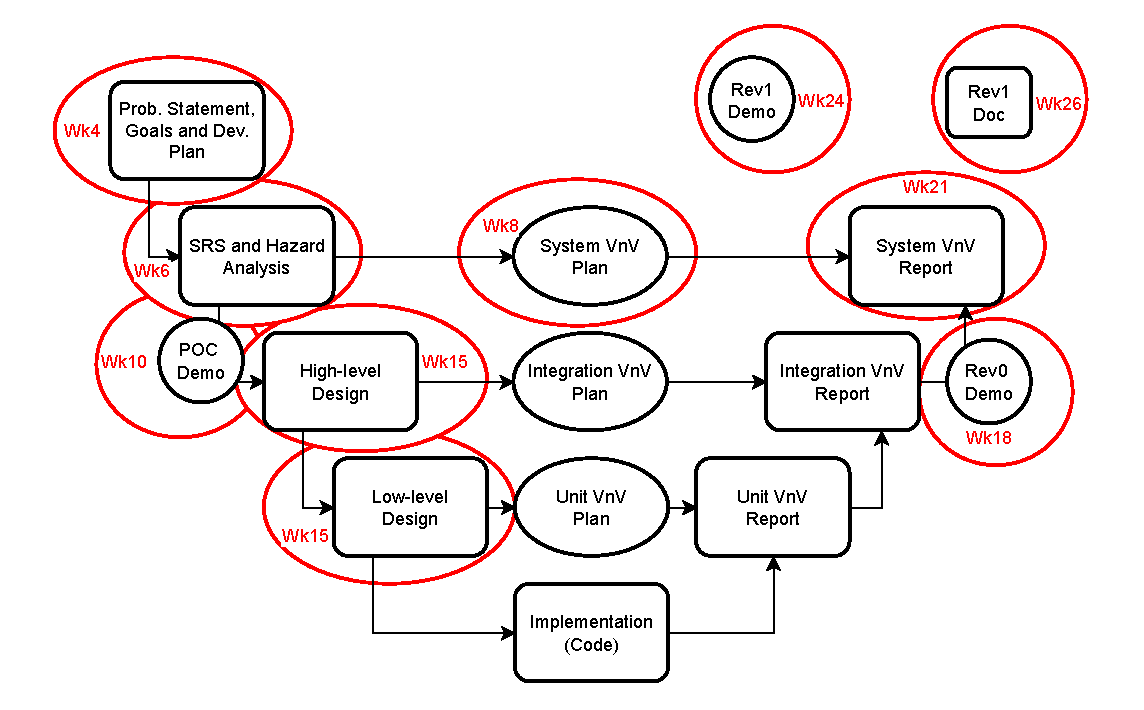
\includegraphics[width=1.1\columnwidth]{./figures/CourseStructure.drawio.pdf}
    }
    \caption{\label{Fig_VModel} V Model Used for Capstone Deliverables}
  \end{center}
\end{figure}
% TODO - redraw the figure if time, and save as pdf
\subsection{Template Repository}

All teams start their project by using the same
%\href{https://github.com/smiths/capTemplate} 
\href{REDACTED Link} {GitHub template repository}. The template repo, summarized
in Figure~\ref{Fig_GitHubTemplate}, contains all the initial infrastructure each
team needs, including the folder structure, text-based template documents and
template issues. The goals of the template are to remove the time team's spend
building their project's infrastructure, and to standardize all the arbitrary
decisions, like folder and document names, between all the teams. The
standardization helps teams when doing peer reviews of each other's work and it
improves communication between the teams, teaching assistants and instructor.
When students have a clear idea of the expectations, they should find it easier
to dive into their project.

\begin{figure}[h!]
  \begin{center}
    {
      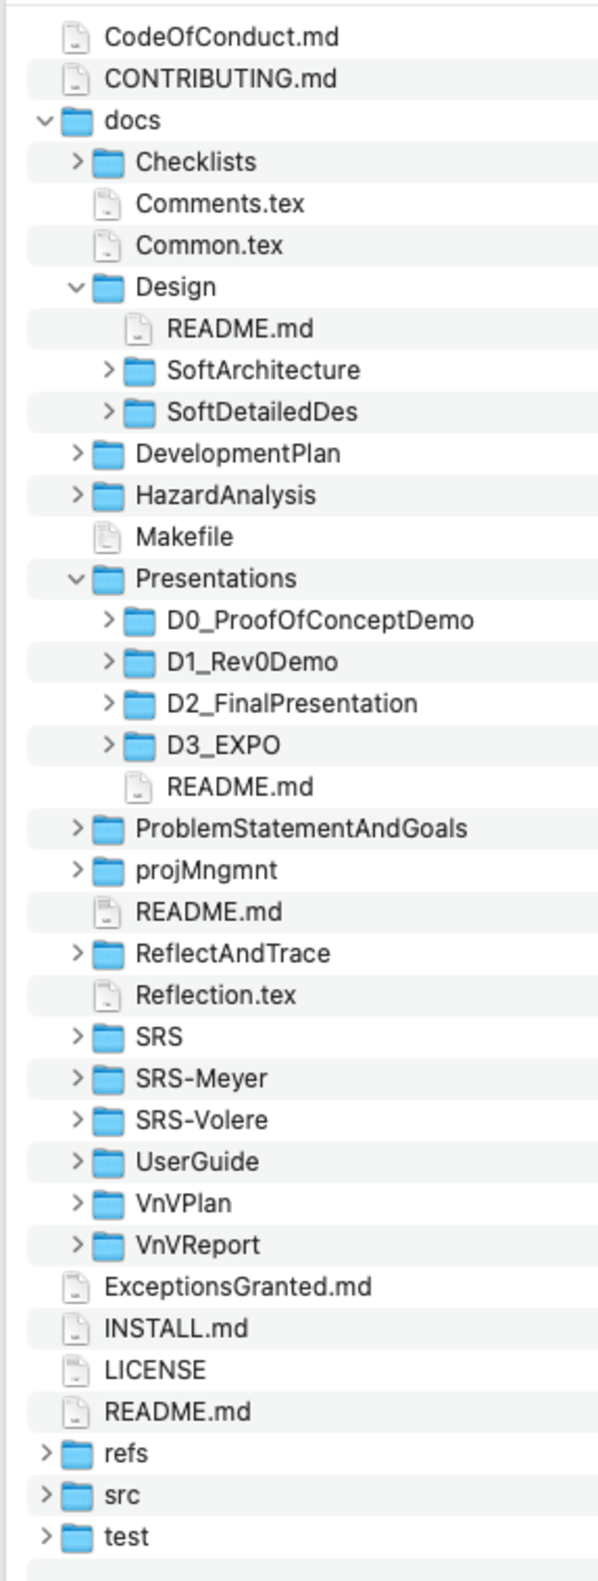
\includegraphics[width=0.7\columnwidth]{./figures/GitHubTemplate}
    }
    \caption{\label{Fig_GitHubTemplate} GitHub Capstone Template}
  \end{center}
\end{figure}

The template documents are written in \LaTeX, although teams are allowed to redo
the template in another text-based format, like markdown, if they wish. Besides
the advantage of separating document appearance from document content, the
text-based format facilitates tracking the productivity of the team members
through git commits, as discussed in Section~\ref{Sec_TeamContribMeasure}. The
documents correspond to the deliverables in Figure~\ref{Fig_VModel}. The
students can use any standard SRS template, including selecting one of the three
options given: SRS (a template for scientific computing
software~\cite{SmithAndLai2005}), SRS-Meyer (a template by Bertrand
Meyer~\cite{Meyer}) and SRS-Voler (the Volere
template~\cite{RobertsonAndRobertson1999Vol}).

For further standardization, the template repo includes
\href{Redact link}
%\href{https://github.com/smiths/capTemplate/tree/main/.github/ISSUE_TEMPLATE}
{four issue templates} for: 1) team meeting agendas; 2) TA-team meeting agendas;
3) supervisor-team meeting agendas; and, 4) lecture attendance.  In addition to
encouraging good organizational habits, the issues are also used to partly
measure the commitment of students to their teams, as discussed in the next
section.

\subsection{Team Contribution Measurement} \label{Sec_TeamContribMeasure}

To improve the distribution of the workload to all team members, we can take
advantage of the quantifiable productivity measures available from git and
GitHub.  Specifically we can use the issue tracker to quantify team meeting
attendance and we can use GitHub insights to count the commits to the main
branch for each team member.  Each team produces a summary table as part of
their \href{REDACT LINK}  
%\href{https://github.com/smiths/capTemplate/tree/main/docs/projMngmnt}
{performance report} before the three demonstrations: POC demo, Rev0 demo and
Rev1 demo (see Figure~\ref{Fig_VModel} for the timing). In the performance
report the team can also record reasons for a team member to appear to perform
poorly on any of the metrics. The hope for explicitly capturing these numbers
will reveal any problems with team collaboration.  Ideally the problems will be
revealed early and improved, but if the problem cannot be dealt with, at least
there will be enough data to assign a fair individual grade to all team members.

- co-author commits

Measures used by team.  Team charter. 
- also survey

\section{Preliminary Data} \label{SecPrelimData}

Look at commits over time, and possibly lines (removing outliers) of code over
time


\subsection{Timeline Comparison}

Timeline comparison

\begin{figure}[h!]
\begin{center}
{
     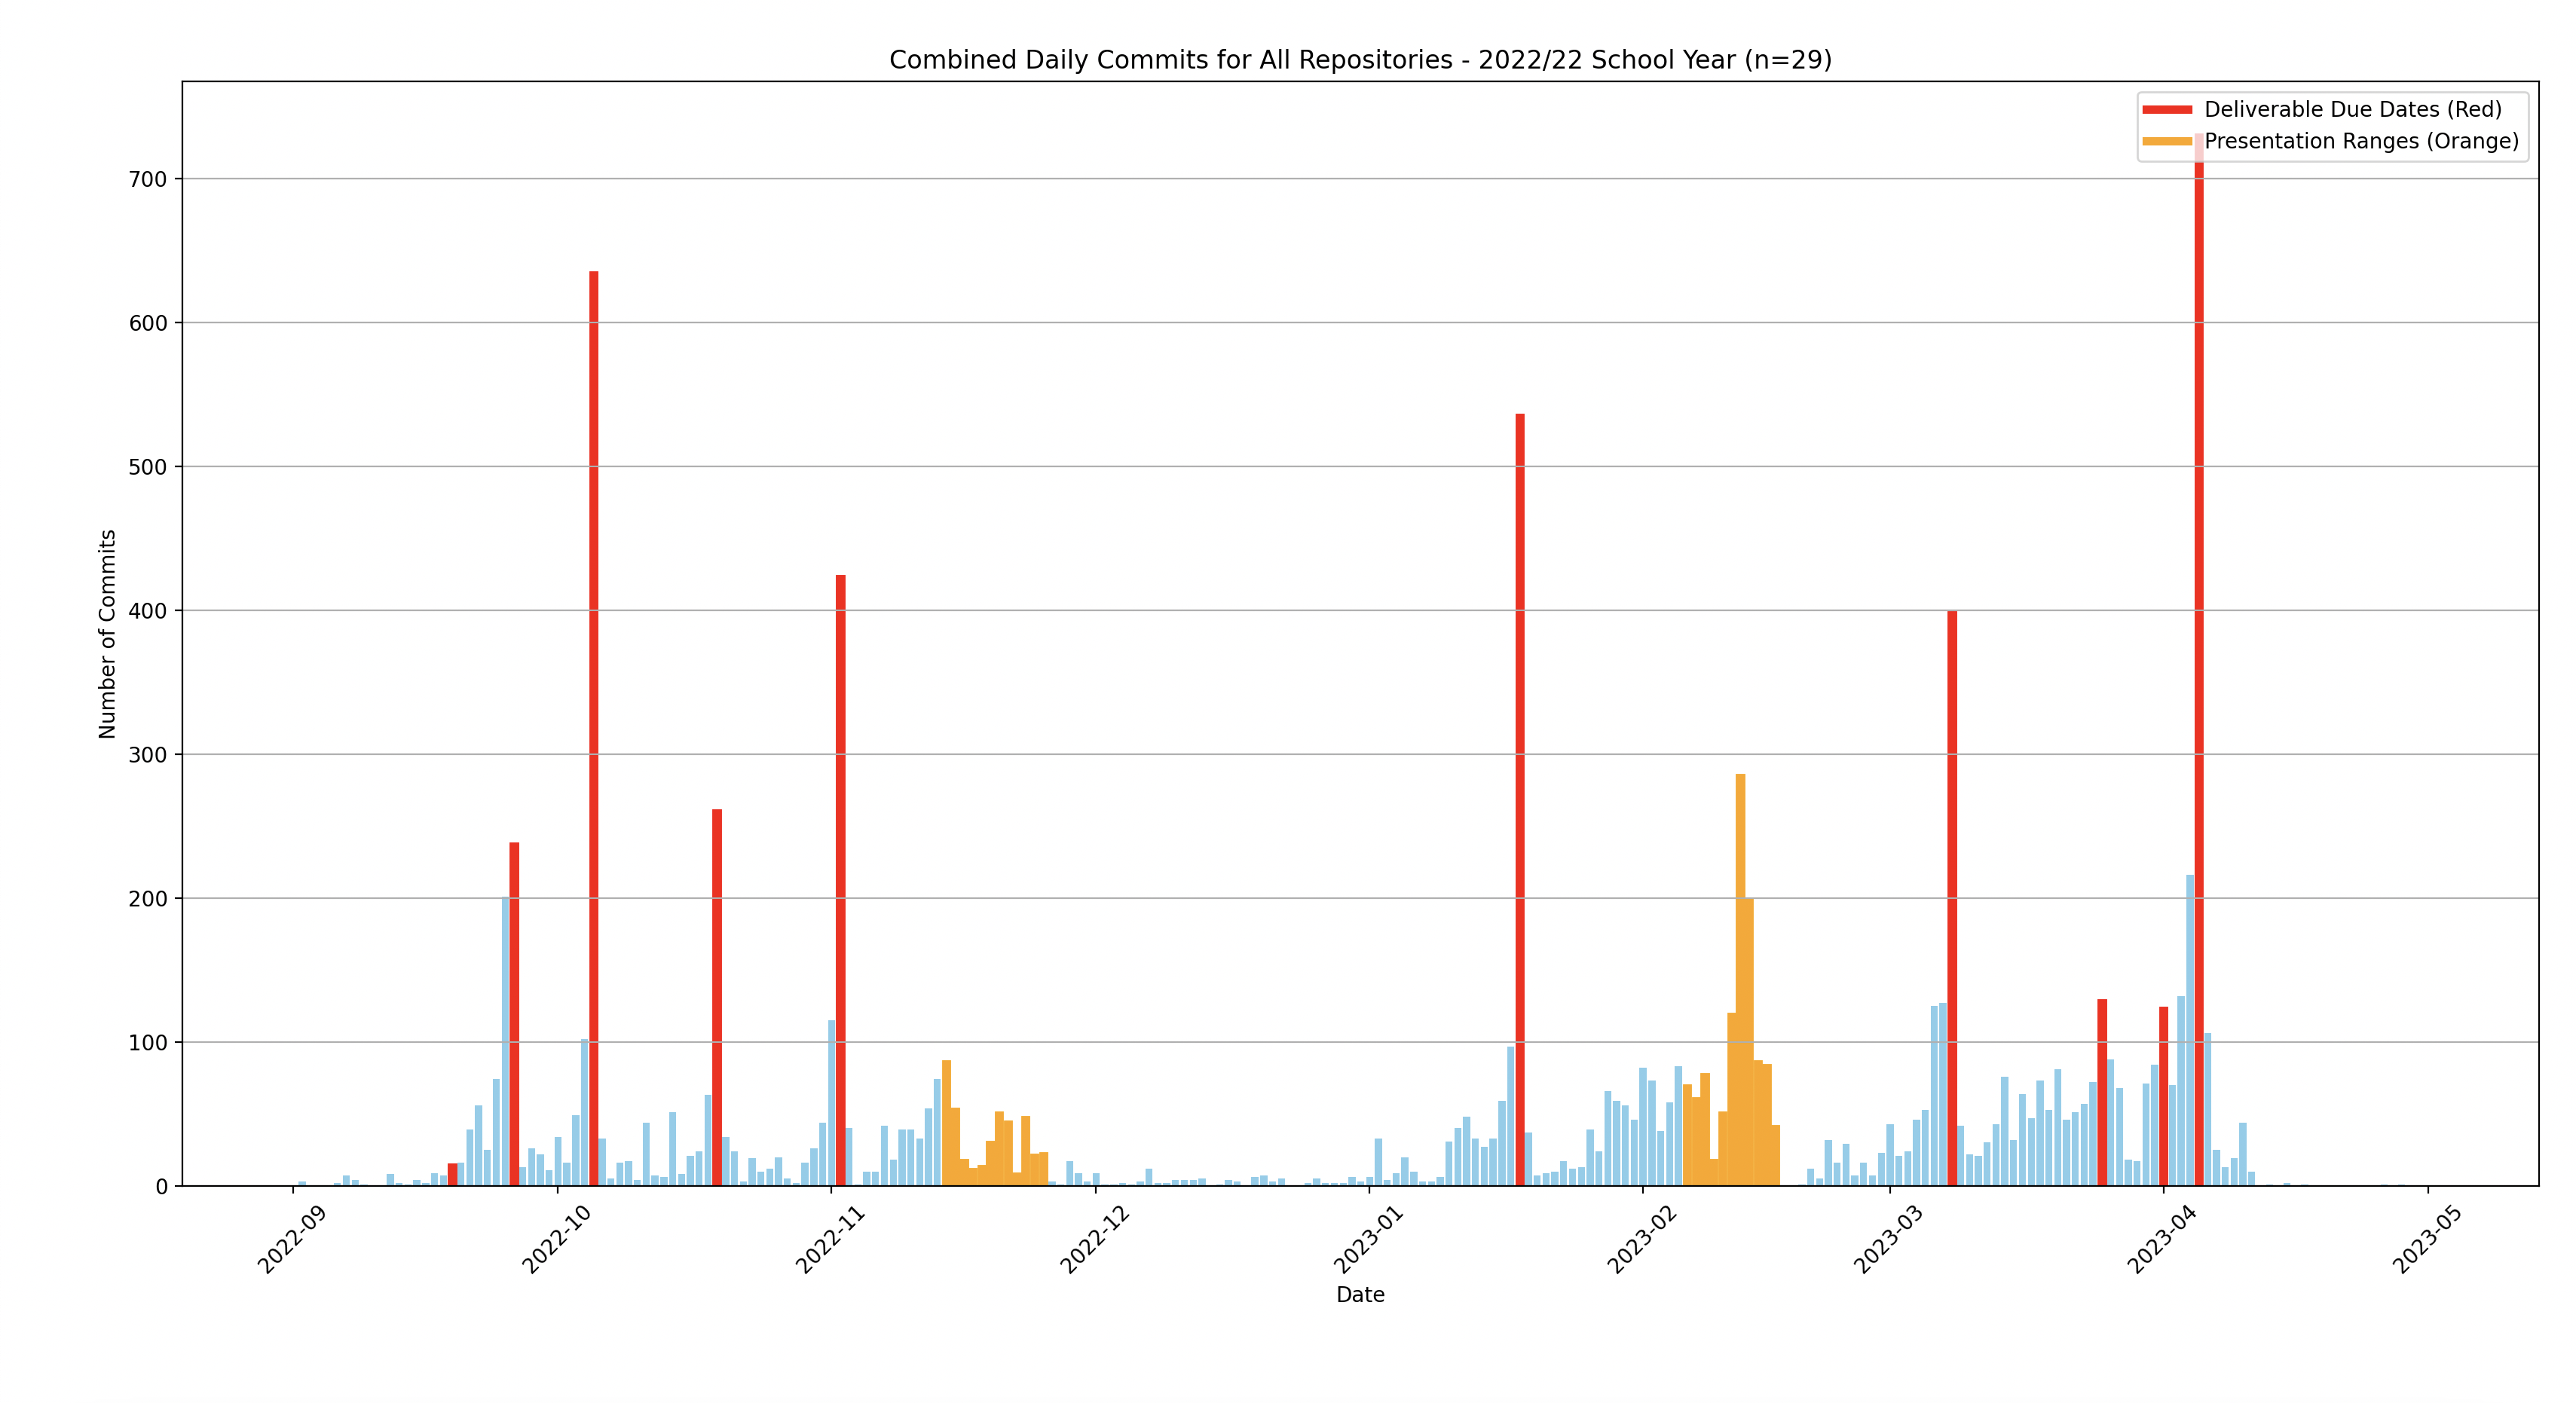
\includegraphics[width=0.75\columnwidth]{./figures/Yr22_23_DailyCommitsTimeline.png}
}
\caption{\label{Fig_22_23Timeline} Timeline of Commits for 2022--2023}
\end{center}
\end{figure}
  
\begin{figure}[h!]
\begin{center}
{
     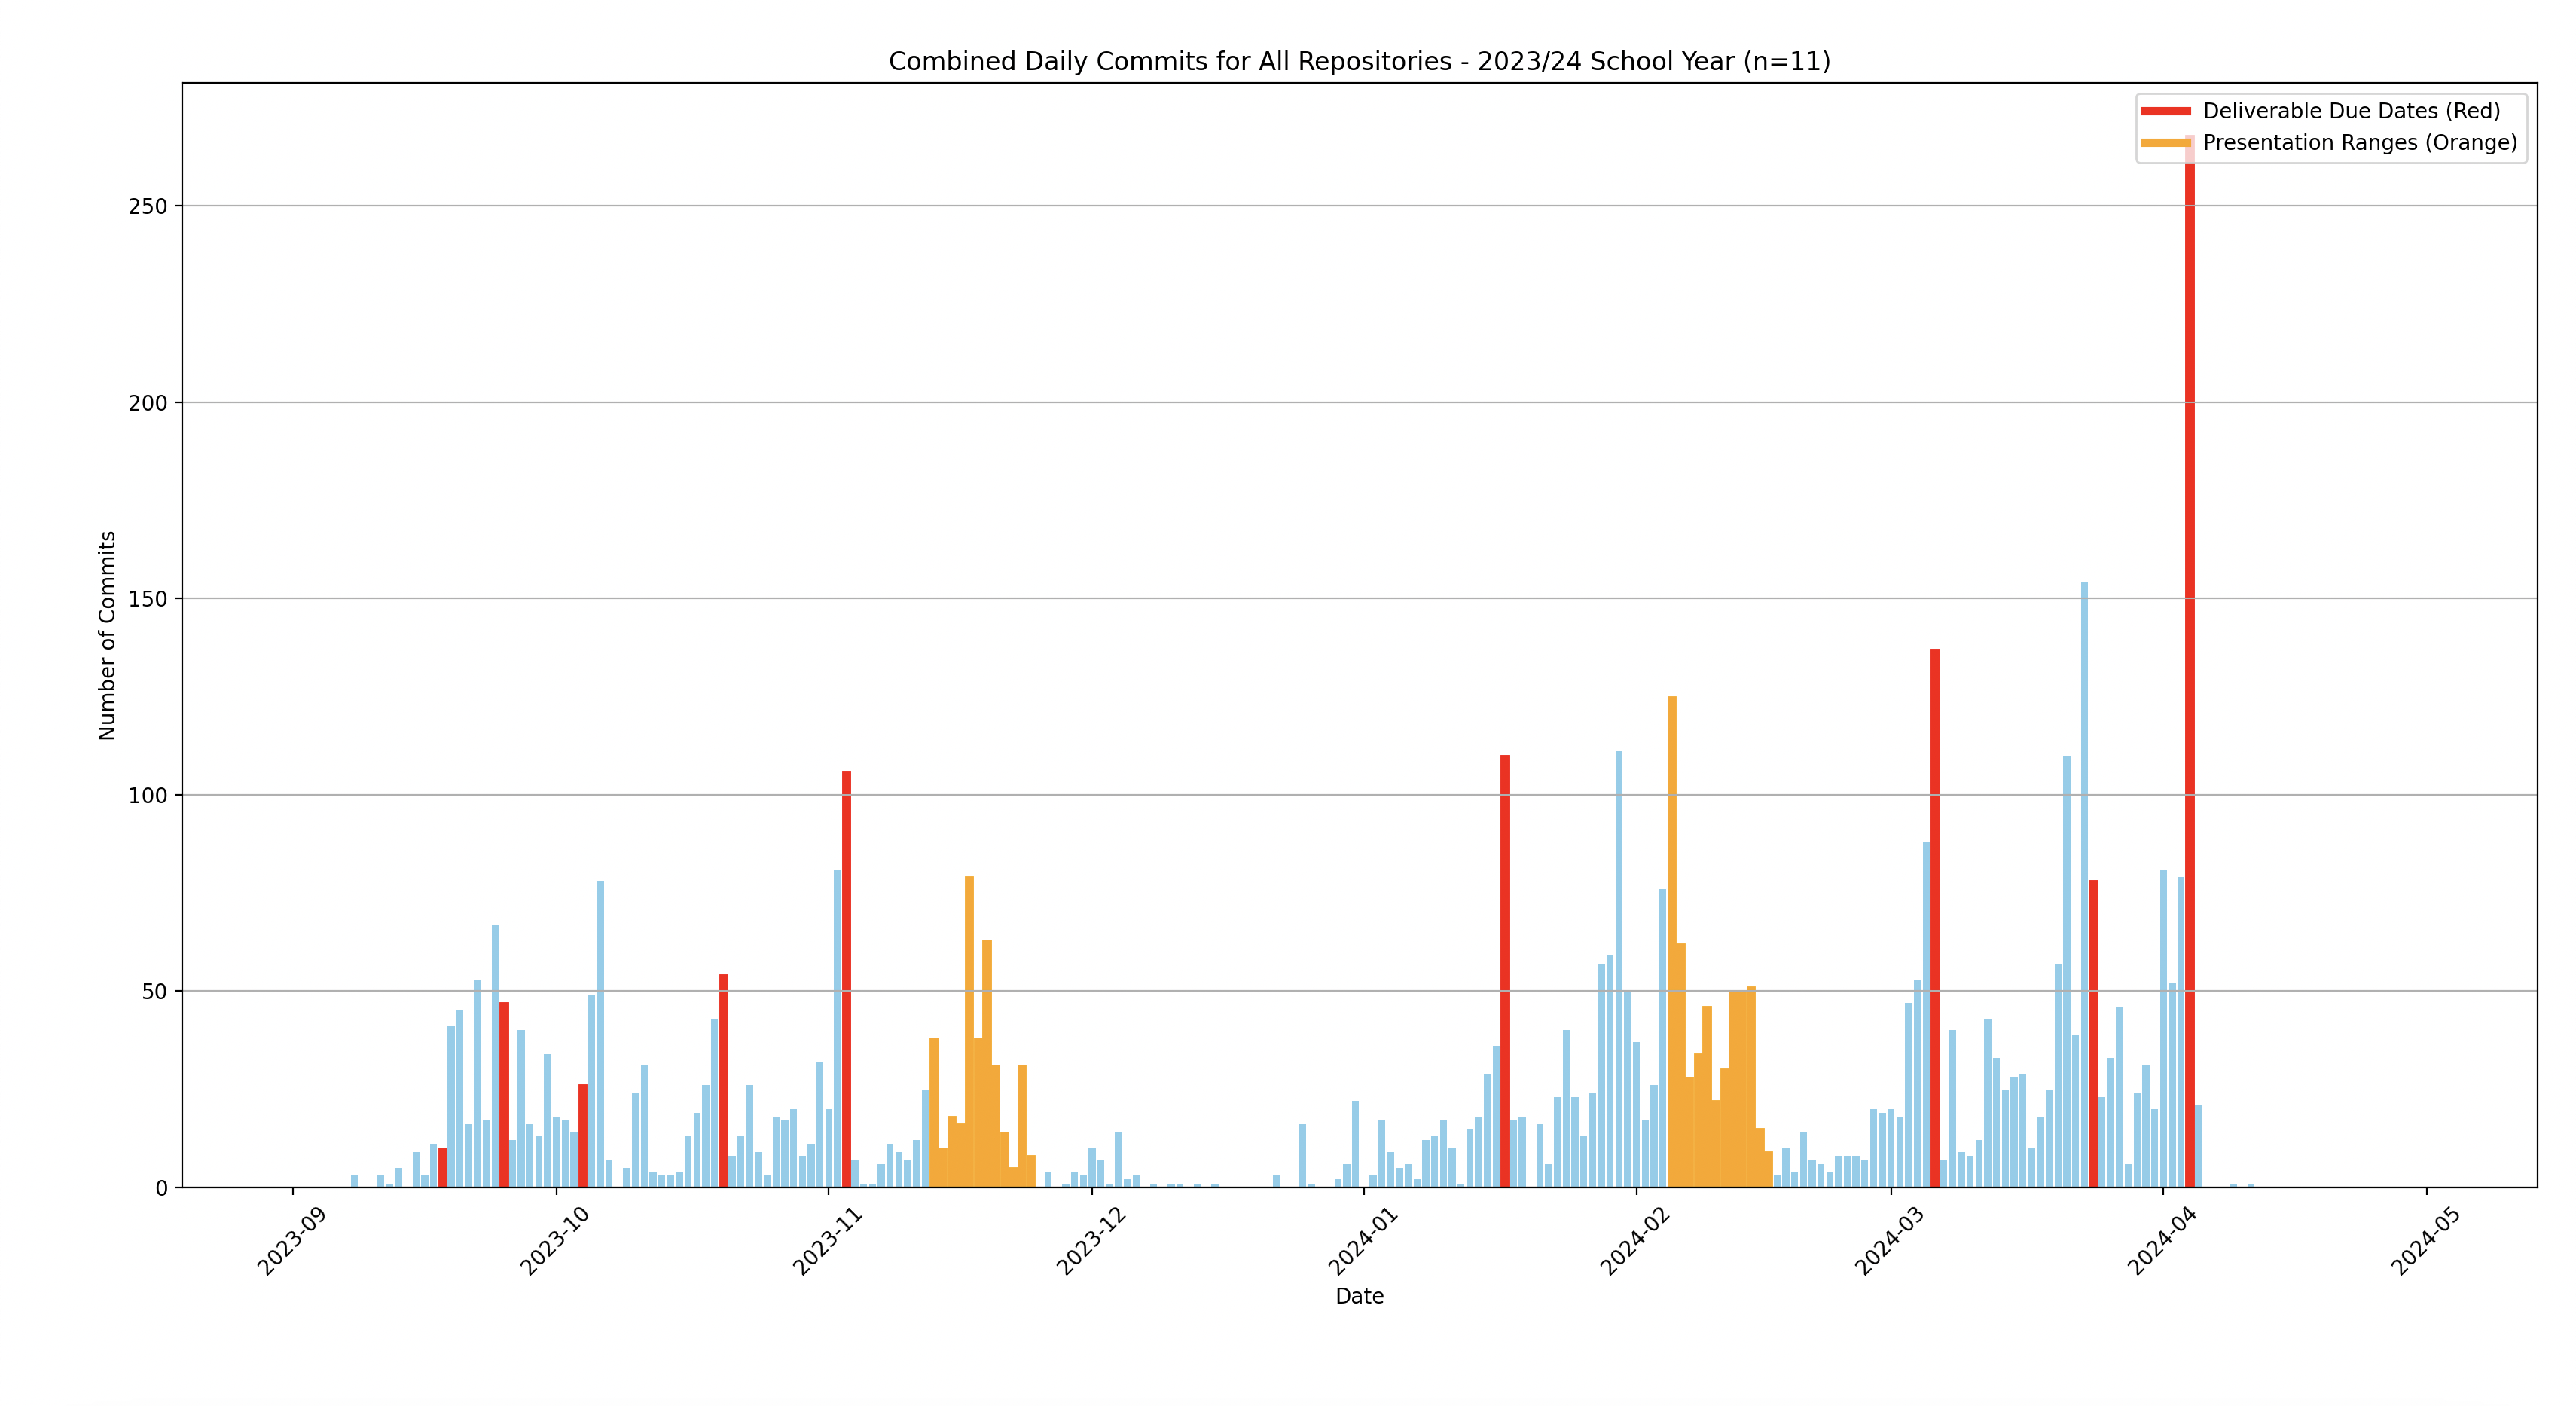
\includegraphics[width=0.75\columnwidth]{./figures/Yr23_24_DailyCommitsTimeline.png}
}
\caption{\label{Fig_23_24Timeline} Timeline of Commits for 2023--2024}
\end{center}
\end{figure}

\subsection{Measuring Fairness}

In order to measure the fairness of work distribution among teammates,
we sought to compute a metric where values range from 0 to 1, and where values
in between contain meaningful information.
Thus, we devised the following \textit{unfairness} metric where $C$:

$$
\text{unfairness}(C) = \frac{ \sum\limits_{c, x \in C, c > x} (c-x)}{(\left|C\right| -
1) \cdot \sum\limits_{c \in C} c}
$$

\noindent where $C$ is the multiset of teammates' numbers of commits to the 
repository.

The metric computes the sum of the difference between each teammate's commits
and those who committed less than them, normalized by the number of teammates
(excluding themselves) and the total number of commits. This yields a value
from 0 to 1, called the \textit{unfairness} metric, where:

\begin{itemize}
  \item 0 indicates that teammates did an equal amount of work
  \item 1 indicates that all the work was done by one teammate
  \item A value between 0 and 1 indicates the proportion of work 
        per person which could have been given to someone who did less work
\end{itemize}

Fairness is defined as $\text{fairness}(C) = 1 - \text{unfairness}(C)$.

For example, if a team with Persons A, B, and C did 10, 5 and 5 commits respectively, then
$\text{unfairness}(\{10,5,5\}) = 0.25$. This is because on average Person A did 5 more commits than
their teammates and thus these 5 commits (out of 20) are considered \textit{unfair work}. The fairness 
value is thus 0.75.

Figs.~\ref{Fig:Fairness22-23} and~\ref{Fig:Fairness23-24} show the fairness values for 
teams in 2022/23 and 2023/24 respectively.

In the future, we will experiment with applying this metric to things other than commits (e.g.~lines of
code written, issues created/closed, etc.), as well as investigating a correlation between
lower fairness values and perceived unfairness according to the teammates themselves. Another
research question would be if having live access to this fairness metric encourages teams to share
work more evenly or simply encourages them to ``game the system'' to increase the value.

\begin{figure}[h]
\centering
\begin{tikzpicture}
\begin{axis}[
    ybar,
    bar width=0.3cm,
    width=0.5\textwidth,
    height=0.4\textwidth,
    symbolic x coords={Flick-Picker/full-stack, marlon4dashen/Hairesthetics, arkinmodi/project-sayyara, jeff-rey-wang/utrition, mehtaj8/Greenway, Tamas-Leung/CodeChamp, HKanwal/kapstone, paezha/PyERT-BLACK, BillNguyen1999/REVITALIZE, RutheniumVI/UnderTree, agentvv/MTOBridge, NicLobo/Capstone-yoGERT, brandonduong/Farming-Matters},
    xtick=\empty,
    nodes near coords = {},
    nodes near coords align={vertical},
    ymin=0,
    ymax=1,
    ylabel={Fairness},
    xlabel={Team},
    enlarge x limits=0.1,
    legend style={at={(0.5,-0.15)},anchor=north,legend columns=-1},
    ymajorgrids=false,
    grid style=dashed,
]
\addplot coordinates {
    (Flick-Picker/full-stack, 0.3562048588312541)
    (marlon4dashen/Hairesthetics, 0.4509090909090909)
    (arkinmodi/project-sayyara, 0.5239228125826064)
    (jeff-rey-wang/utrition, 0.541871921182266)
    (mehtaj8/Greenway, 0.5447537473233405)
    (Tamas-Leung/CodeChamp, 0.5865051903114187)
    (HKanwal/kapstone, 0.6448184233835252)
    (paezha/PyERT-BLACK, 0.6550335570469799)
    (BillNguyen1999/REVITALIZE, 0.6649842271293376)
    (RutheniumVI/UnderTree, 0.7277227722772277)
    (agentvv/MTOBridge, 0.751219512195122)
    (NicLobo/Capstone-yoGERT, 0.8527835051546392)
    (brandonduong/Farming-Matters, 0.8534278959810875)
};
\end{axis}
\end{tikzpicture}
\caption{Fairness of Commits Per Team 2022/23 [n=13] (Mean: 0.63, Stddev: 0.15)}\label{Fig:Fairness22-23}
\end{figure}

\begin{figure}[h]
\centering
\begin{tikzpicture}
\begin{axis}[
    ybar,
    bar width=0.3cm,
    width=0.5\textwidth,
    height=0.4\textwidth,
    symbolic x coords={r-yeh/grocery-spending-tracker, DangJustin/CapstoneProject, Tusharagg1/chest-x-ray-ai, d-akselrod/SweatSmart, InfiniView-AI/MotionMingle, stanreee/sign-language-learning, RishiVaya/capstone-12, MichaelBreau/nlp-mentalhealth, SammyG7/Mac-AR, beatlepie/4G06CapstoneProjectTeam2, katrina799/4G06CapstoneProjectT5},
    xtick=\empty,
    nodes near coords = {},
    nodes near coords align={vertical},
    ymin=0,
    ymax=1,
    ylabel={Fairness},
    xlabel={Team},
    enlarge x limits=0.1,
    legend style={at={(0.5,-0.15)},anchor=north,legend columns=-1},
    ymajorgrids=false,
    grid style=dashed,
]
\addplot coordinates {
    (r-yeh/grocery-spending-tracker, 0.3200145958766648)
    (DangJustin/CapstoneProject, 0.40943193997856375)
    (Tusharagg1/chest-x-ray-ai, 0.42666666666666664)
    (d-akselrod/SweatSmart, 0.5186666666666666)
    (InfiniView-AI/MotionMingle, 0.525830258302583)
    (stanreee/sign-language-learning, 0.5411013567438148)
    (RishiVaya/capstone-12, 0.6203860480866915)
    (MichaelBreau/nlp-mentalhealth, 0.6298472385428907)
    (SammyG7/Mac-AR, 0.6379532486655624)
    (beatlepie/4G06CapstoneProjectTeam2, 0.6618181818181819)
    (katrina799/4G06CapstoneProjectT5, 0.7661417322834646)
};
\end{axis}
\end{tikzpicture}
\caption{Fairness of Commits Per Team 2023/24 [n=11] (Mean: 0.55, Stddev: 0.13)}\label{Fig:Fairness23-24}
\end{figure}

\section{Proposed Experiment} \label{SecProposedExperiment}

blurb

\subsection{Experiment}

Start with research questions.

Collect the same data as in Section~\ref{SecPrelimData} and conduct focus groups
in all three CAS capstone courses (SE, CS and TRON).  

\subsection{Threats to validity}

\begin{itemize}
    \item Multiple changes are made to the course, so it is difficult to
    determine which change influences the student behaviour.  The focus group
    should hopefully tease that out.
    \item Comparing different courses with different instructors, different
    backgrounds for students, etc.
    \item Not a controlled experiment - introducing more than one change into
    the course.  The changes are related because the productivity metrics would
    not be possible without a version control system.
    \item The interventions proposed here might behave differently for a
    capstone course that follows a different structure
    (Section~\ref{Sec_Structure}).
\end{itemize}

\section{Concluding Remarks} \label{SecConclusions}

The template presented here is for the capstone course under discussion; the
template could be forked and modified to match the needs of a different capstone
course.

\section*{Acknowledgements}

If any.

\bibliographystyle{IEEEtran}
\bibliography{SmithEtAl2024_CSEEnT}

\end{document}
